\chapter{Datasets}

Optical Character Recognition requires data as any other machine learning task. Data are usually divided in two main types - scene and synthetic. Scene datasets contains photographs of real world objects and sceneries where some text occurres, for example shop signs, road signs or car plates. Synthetic dataset are automatically generated images where words are chosen from a extensive dictionary, a font is picked for each word and some sort of deformation is applied. It can be a text distortion to make the text curved or projectively altered, as well as blurring or lighting changes that make the text less obvious for the detector.

Synthetic datasets are usually used for training the models, because it is easier to generate millions of synthetic images rather than to take even one hundredth of a such number of photographs. Needless to say that when generating an image, the ground truth is known and can be saved during the generation process while photographs have to be manually labeled which takes time and might be inaccurate or automatically labeled which also often leads to many mistakes. Scene datasets are then used for testing purposes or for fine tuning a pretrained model.

In the following section sample datasets are introduced. To begin with synthetic dataset MJSynth is a very important dataset because it consists of almost 9 million images covering 90,000 English words. It includes data only for recognition which means that one image has only one word and border of the image  represents the word bounding rectangle.\cite{mjsynth}. Another synthetic dataset is called SynthText and contains 800 thousand images with approximately 8 million word instances written on the images \cite{synthtext}. Three scene text datasets were created for International Conference on Document Analysis and Recognition (ICDAR) competition. Sets ICDAR03, ICDAR13 and ICDAR15 were used in competitions in years 2003, 2013 and 2015, respectively. First two ICDAR datasets include only horizontal text, text of various orientation appears  in set from 2015 \cite{raisi2020text}. Another widely used dataset is The Street View Text (SVT) which contains images with text harvested from Google Street View \cite{svt}. SVT and most other scene text datasets offers mainly frontal text with minimal perspective distorision. However, perspective text is frequent in real life applications of OCR for example previously mentioned street photographs, where it is impossible to capture every visible text from frontal view. Thus Phan et. al \cite{svtp} created a new StreetViewText-Perspective derived from SVT, it shows the same places as SVT but from different perspective. Another dataset CUT80 focuses on curved text as well as CTW1500 dataset. For text recognition there exist for example IIIT5k dataset containing 5000 cropped images harvested from Google image search. It combines both scene text images and born-digital images \cite{IIIT}. One of the most widely used dataset is COCO-Text which includes over 60,000 images with almost 250,000 word instances \cite{coco}.

Datasets that were used for comparission of detection and recognition methods, namely, SCUT-CTW1500 dataset, Kaist Scene Text Database, Born-Digital Images, are described in more detail below. 


\section{SCUT-CTW1500 dataset}

SCUT-CTW1500 dataset contains exactly 1500 images of real-world, scene text in English language. Sample images can be seen in Figure \ref*{Obr:Dctw}. The key feature of this dataset is that each image contains horizonally aligned text, multioriented text and curved text. There are cases where the curvature is only slight and cases where text forms a circle with letter upside down. Recognizing multi-oriented and curved text is more of a challenge than pure horizontal text. This dataset is split to train and test data. Two thirds of dataset thus one tousand images for training and five hundred for testing. According to the description of this dataset on relevant GitHub repository dataset was manually labeled and lately corrected, therefore labels seem to be very accurate. However for example ground truth for image 1313.jpg misses all occurences of letter I, as the depicted font was probably misread.\cite{ctw,ctw2}

The ground truth for train data are in XML format and each file carries information about the file name of respective image file, text information -- i.e., words in a text line, 14 coordinates of a bounding polygon and coordinates, height and width of a circumsribed rectangle. Later the authors added coordinates of center point of each English letter to be used as detection ground truth. The ground truth of test data is in simple text file (TXT) and contains only 14 coordinates of the bounding polygon and a text which is within that region. There is a minor issue with labels that it usually contains a full text line with multiple words and coordinates are not assigned to individual words but to text region as whole. Most end-to-end system detect words rather than groups of corresponding words. This fact needs to be taken into account when evaluating results.

\begin{figure}[hbtp]
    \centering
    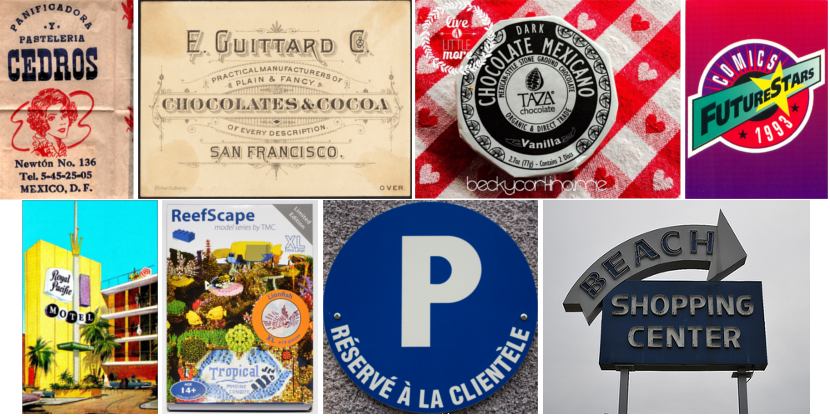
\includegraphics[scale=0.4]{obrazky/Dataset_ctw.png}
    \caption{Sample images of SCUT-CTW1500 dataset.}
    \label{Obr:Dctw}
\end{figure}

\section{KAIST Scene Text Database}

This dataset contains 3000 images of photographed text. It can be divided into three major catgories -- text of Korean language, English language and mixed languages. As I concentrate on text in latin script in this paper further information relates to the English language dataset. The number of images is then reduced to less than four hundred images. Figure \ref*{Obr:Dkaist} shows few samples of this dataset. Photographed objects are mostly shop banners or parts of magazine front pages. Photographs were either taken by a high-resolution digital camera or a low-resolution mobile phone camera.\cite{kaist} Each photography has a ground truth description and a bitmap image. In the bitmap file only text is highlighted (by white or red color) and everything else apart from text is set as black. Ground truth files are in XML format and includes a name of an image, its resolution and bounding box for each word and also a bounding box for each letter of the word.

To use this dataset for testing and training the XML ground truth needed to be converted to string and int values. I wrote a parser, that combines letters to form a word that is within a given bounding box. I changed the notation of bounding boxes from one coordinate, width and height attributes to two top left and bottom right coordinates.

Unfortunately this dataset has few errors in filenames of corresponding files or in the content of XML files. Usually these are only typos, however they prevent automatic preprocessing of dataset. Due to this problem these mistakes need to be found and  manually corrected. Also there is a small number of ground truth XML file with fully missing data. 
Despite these shortcomings this dataset is useful because of the bitmap files. This allows to compare results of both images affected by shooting conditions and images dependent only on font and position.

\begin{figure}[hbtp]
    \centering
    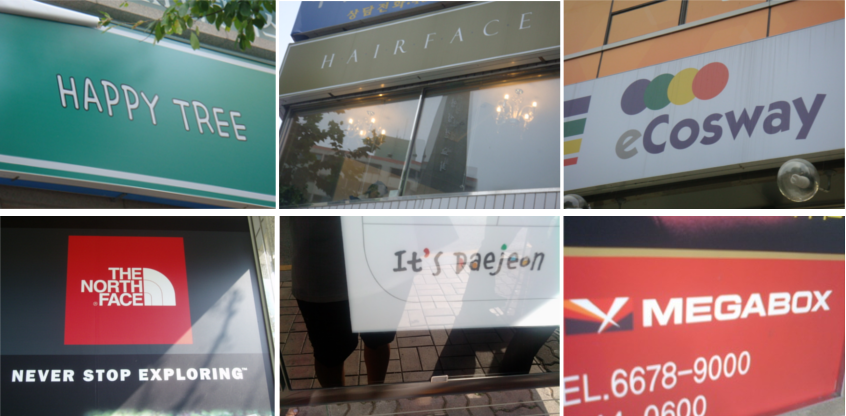
\includegraphics[scale=0.4]{obrazky/Dataset_kaist.png}
    \caption{Sample images of KAIST Scene Text Database dataset.}
    \label{Obr:Dkaist}
\end{figure}

\section{Born-Digital Images}

Born-Digital Images contains data of images with text that can be found on various websites. Samples of this dataset can be found is in Figure \ref*{Obr:Dbd}. There are mostly advertisments, company logos or website headers. Such pictures cannot be classified neither as real scene dataset, neither as synthetic one. On one hand  this dataset shares with scene datasets the variability in font styles and sizes, different text orientations and complex colour placement. On the other hand it differs in size because low resolution is significant in smooth and fast loading on websites. Also no noise is present due to lighting conditions. Geometrical deformations that result when capturing a real scene with camera also do not appear here. However compression to lower resolution can lead to artefacts and aliasing. In general we can say that letters are more clearly visible than in photographed text as easy readability is crucial in successful advertising.\cite{born-digital1}

The dataset is available for download from the website of Robust Reading Competition. First version was published in 2011 and revised two years later, it contains separate dataset for text localization, segmentation and then for word recognition. In 2015 they published an end-to-end dataset with ground truth for all tasks. The dataset is split in training and testing data. However, ground truth for testing data contains only a possible vocabulary of words in images and no coordinates. This might be due to the fact that the competition might be still ongoing or there was not a sufficent demand for complete ground truth. As for training data, each image has a corresponding TXT file with coordinates of four vertices of bounding rectangle and a word. Text lines are separated and the text within rectangle is always one word. Unfortunately, there are quite a few missing words, usually words that have two or less characters. This can affect the evaluation when the model finds such a short, missing word.\cite{born-digital1}

\begin{figure}[hbtp]
    \centering
    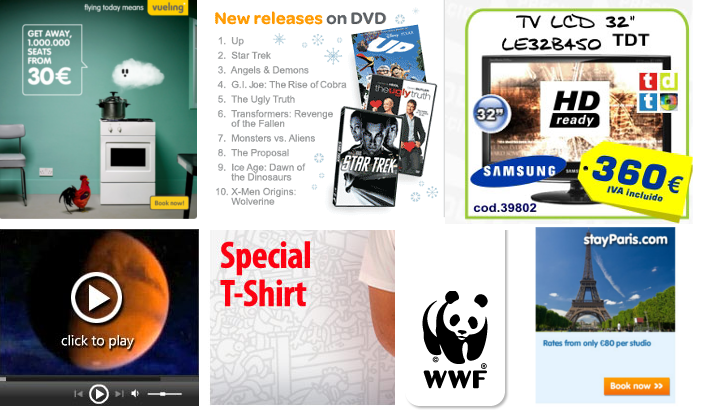
\includegraphics[scale=0.4]{obrazky/Dataset_born-digital.png}
    \caption{Sample images of Born-Digital Images dataset.}
    \label{Obr:Dbd}
\end{figure}


\section{Wien TU dataset}

